\documentclass[11pt,a4paper]{article}
%\usepackage[toc,page]{appendix}
\usepackage{graphicx}
\usepackage[a4paper]{geometry}
\usepackage{xcolor}
\usepackage{fancyhdr}
\usepackage{float}
\usepackage{setspace}
\usepackage[absolute]{textpos}
\usepackage{epstopdf}
%\usepackage[]{mcode} 	% To include matlab code
\usepackage{capt-of}
\usepackage{enumerate}
\usepackage{lastpage}
\usepackage{booktabs}
\usepackage{longtable}
\usepackage{array}
\renewcommand{\arraystretch}{1.5}

\usepackage[english]{babel}
\usepackage[utf8]{inputenc}
\usepackage{amsmath}
\usepackage{amsfonts}
\usepackage{graphicx}
\usepackage[colorinlistoftodos]{todonotes}
\usepackage{algorithm}
\usepackage{algpseudocode}

\usepackage{amsmath}
\usepackage{algorithm}
%\usepackage[noend]{algpseudocode}
\makeatletter
\def\BState{\State\hskip-\ALG@thistlm}
\makeatother

\usepackage{amsmath}
\usepackage{amsfonts}
\usepackage{amssymb}
\usepackage{eurosym}

% Header
\setlength{\headheight}{30pt}
\newgeometry{top=2.5cm, bottom = 1.5cm, left=2cm, right=2cm}
\pagestyle{fancy} 
\lhead{\includegraphics[height=0.8cm]{figures/{tue_logo}.png}}
%\lfoot{Group 4 - ``CASE"-HENK}
\cfoot{~}
\rfoot{Page \thepage ~of \pageref{LastPage}}

\usepackage{cleveref}
% Change cleveref reference eq. to equation same for figure
\crefname{equation}{equation}{equations}
\crefname{figure}{figure}{figures}
\crefname{table}{table}{tables}

% Change Section numbering to Problem 1
%\renewcommand{\thesection}{Problem \arabic{section}.}

\begin{document}
%\begin{titlepage}
%\vspace*{100pt}
%\begin{figure}
%\centering
%\includegraphics[width=0.5\textwidth]{figures/TUelogozondertekst}
%\end{figure}
%\begin{center}
%{ \huge \bfseries 4AT100 Automotive Systems Engineering Project\\[0.4cm] }
%\textsc{\Large Concept Project Plan}\\[0.5cm]
%
%\end{center}
%
%\vfill
%
%\renewcommand{\arraystretch}{1}
%
%\begin{flushleft} \large
%\begin{tabular}{l}
%Project Coordinators:\\
%Dr.Ir. A. van de Mortel-Fronczak (Asia) \\
%Dr.Ir. I. Barosan (Ion) \\
%\end{tabular}
%\end{flushleft}
%
%\begin{flushleft} \large
%\begin{tabular}{l l l l}
%Tutor: & & & \\
%L. Kefalidis (Lazaros) & & & \\
%& & & \\
%Authors:\hspace{30mm} 	& \hspace{35mm}	& \hspace{55mm} 	    		& 			\\
%S. Forno (Simone) 		& ​0978942		& T. de Mor\'ee (Tim)			& 0944052 	\\
%R.M.A. Goris (Rob) 		& 0808822		& T.M.A. van de Wiel (Thijs)	​& 0824530 	\\
%B.S. Haarsma (Bouke) 	& 0751757​		& H. Wils (Hielke) 				& 0807014 	\\
%\end{tabular}
%\end{flushleft}
%
%\begin{flushleft} \large
%\begin{tabular}{l}
%MSc. Programme Automotive Technology \\
%Eindhoven University of Technology \\
%\end{tabular}
%\end{flushleft}
%
%\begin{flushleft} \large
%\begin{tabular}{l}
%\today \hspace{8.4cm} Group 4 ``CASE"-HENK \\
%\end{tabular}
%\end{flushleft}
%
%\renewcommand{\arraystretch}{1.5}
%
%\end{titlepage}

\newgeometry{top=2.5cm, bottom = 3cm, left=2cm, right=2cm}

%\newpage
%
%\setcounter{tocdepth}{2}
%
%\tableofcontents
%\newpage


%------------------------------------------------

\section{Results} \label{sec:res}




\section{To do`s} \label{sec:todos}
\begin{itemize}
\item Make the Husky follow first straight path, using the a simple navigation goal \textbf{solved}. 
\item solve the roslaunch error - to do it tonight 27.09 - \textbf{solved}
\item Get the same result from the simple-navigation-goal with the \textbf{global planner} - implies to create a .txt file in Matlab. Test the simple "go straight one meter" file
\item for today \textbf{4 Ott} learn the Navig Stack book tutorial
\end{itemize}


\section{Achieved}

\begin{itemize}
\item Executable of the simple-navigation-goal found under /simon-ws/devel/lib/simple-navigation-goals. The executable is in place, running the node with \textbf{rosrun simple-navigation-goals simple-navigation-goals} runs the executable. The robot moves one meter forward. 
\item Checking for the odometry on the topic \textbf{/odometry/filtered} shows up the results in Figure \ref{fig:odom_filtered}, this shows a \textbf{20 percent less} in the value of the odometry filtered (Ekf fusion of Encoders and IMU sensors), the same holds for the \textbf{pure odometry} of the topic \textbf{husky-velocity-controller/odom}. 
\item Checking for the \textbf{amcl-pose} topic, this shows even a lower value, see Figure 


\end{itemize}


\begin{figure}[!htb]
	\center
	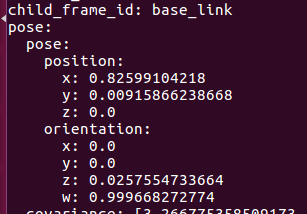
\includegraphics[width=.4\textwidth]{figures/odom_filtered.png}
	\caption{Odometry filtered sending the base-link a 1 meter forward goal}
	\label{fig:odom_filtered}
\end{figure}

\begin{figure}[!htb]
	\center
	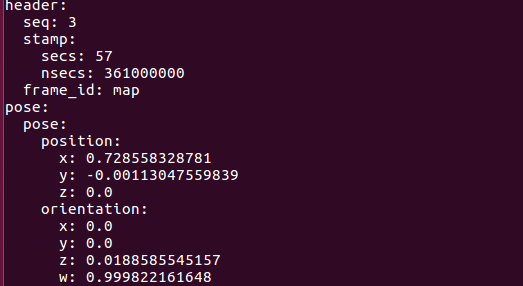
\includegraphics[width=.4\textwidth]{figures/amcl_pose.png}
	\caption{amcl-pose result}
	\label{fig:amcl_pose}
\end{figure}



\section{Comments on Sriram meeting - planner and navigation} \label{sriram}

\begin{itemize}
\item According to the transformation tree from parents to child we find \textbf{map}, \textbf{odom}, \textbf{base}, \textbf{lasercan}. When constructing the map using Gmapping, the reference 0 0 0 is where the mapping process starts, then this is reflected into the Amcl node. So the map frame is 0 0 0 if the Gmapping has started in 0 for each coordinate. So the map frame is \textbf{fixed and global} wrt the map while the odom is \textbf{movable and local} wrt to the base link. 
\end{itemize}


\section{What are msgs}

Nodes communicate with each other by publishing messages to topics. A message is a simple data structure, comprising typed fields. Standard primitive types (integer, floating point, boolean, etc.). There are specific files of a messsage called \textbf{msg}, simple text files specifying the data structure of the message. Example: std{\_}msgs/msg/String.msg the message has the type std{\_}msg/string. The ROS builds the msgs from the msgs file into \textbf{source} code. New data types .msgs can be created in my own package, under the folder \textbf{msg}. When the message is included Ex: move{\_}base{\_}msgs/MoveBaseAction.h, the header file is used to add the timestamp, frame, and so on. This allows messages to be numbered so that we can know who is sending the message. By adding \textbf{rosbuild{\_}add{\_}executable}, this line will create an execut in the \textbf{bin} folder !
 
\section{Understanding the transforms - base{\_}link, odom, map}
Reading this link http://www.ros.org/reps/rep-0105.html-coordinate-frames, the error of Figure \ref{fig:odom_filtered} and \ref{fig:amcl_pose} are due to lack of parameters change in the amcl !!

\section{Further notes on the Navigation Stack following ROS book} 

This sec

\end{document}



% == TABLE ==
%begin{table}[h!]
 % \centering
  %\caption{Caption for the table.}
 % \label{tab:table1}
 % \begin{tabular}{ccc}
 %   \toprule
  %  Some & actual & content\\
   % \midrule
   % prettifies & the & content\\
   % as & well & as\\
  %  using & the & booktabs package\\
  %   \bottomrule
  %\end{tabular}
%\end{table}


% === ALGORITHM == 

\iffalse % multi-comment tool
\begin{algorithm}[!h]
   \caption{Kirsch, Rohig algorithm}
    \begin{algorithmic}[1]
    	\State $St-1 = St$
        \For{$i = 1$ to $N$} \Comment{With N the number of particles in the filter set by maxparticle parameter}
            \State $Spread $ $particles$ $in$ $the$ $anchorbox$ $with$ $equations$ $1)$ $and$ $2)$ $of$ $[3]$ \Comment{This step is called $Global$ $Localization$}
            
            \State $xt[n] = p(xt|xt-1,ut)$ \Comment{Motion update - sample the particles from the motion update of the robot and move forward to estimate the error model functions}
            
        	\State $wt[n] = p(dnanoLOC|si)*p(dlaser|si)$ \Comment{Measurement update - si are the particles set with i the i-th index}
        	\State $St = St + <xt,wt>$ \Comment{add the state and weight to the total state space}
        	
        	\State $Perform$ $resampling$
        \EndFor
    \State $Return$ $St$

\end{algorithmic}
\end{algorithm}
\fi


\iffalse

\begin{figure}[!htb]
    \centering
    \begin{minipage}{.5\textwidth}
        \centering
        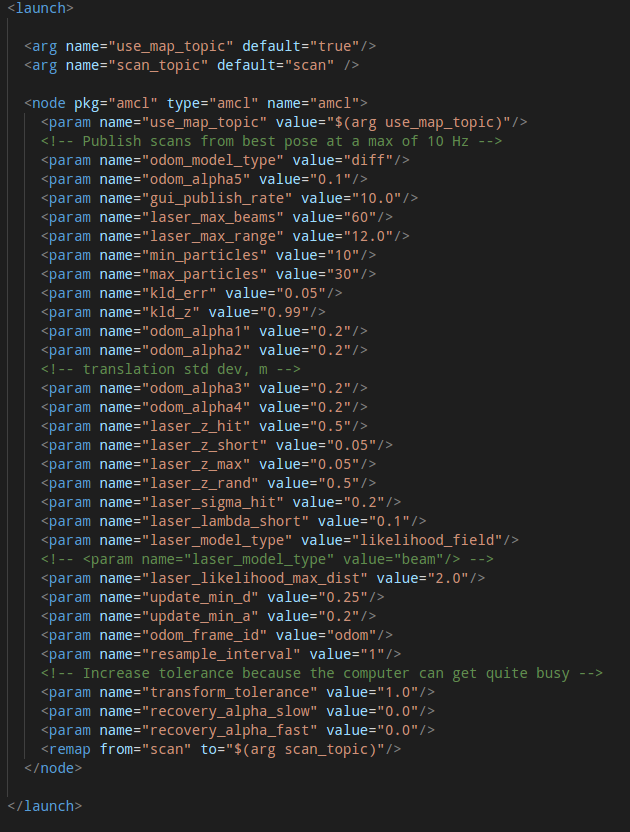
\includegraphics[width=0.7\linewidth, height=0.2\textheight]{figures/amcl_param}
        \caption{The $amcl$ tunable parameters}
        \label{fig:amcl_param}
    \end{minipage}%
    \begin{minipage}{0.5\textwidth}
        \centering
        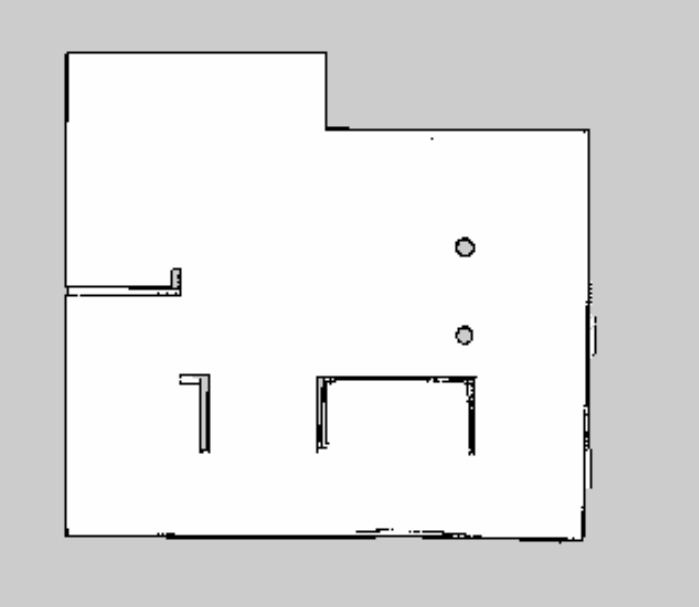
\includegraphics[width=0.7\linewidth, height=0.2\textheight]{figures/my_amcl_gmapping}
        \caption{Result of the Gmapping for the simple indoor environment}
        \label{fig:myamcl_map}
    \end{minipage}
 \end{figure}
 
 
 
 \begin{figure}[!htb]
	\center
	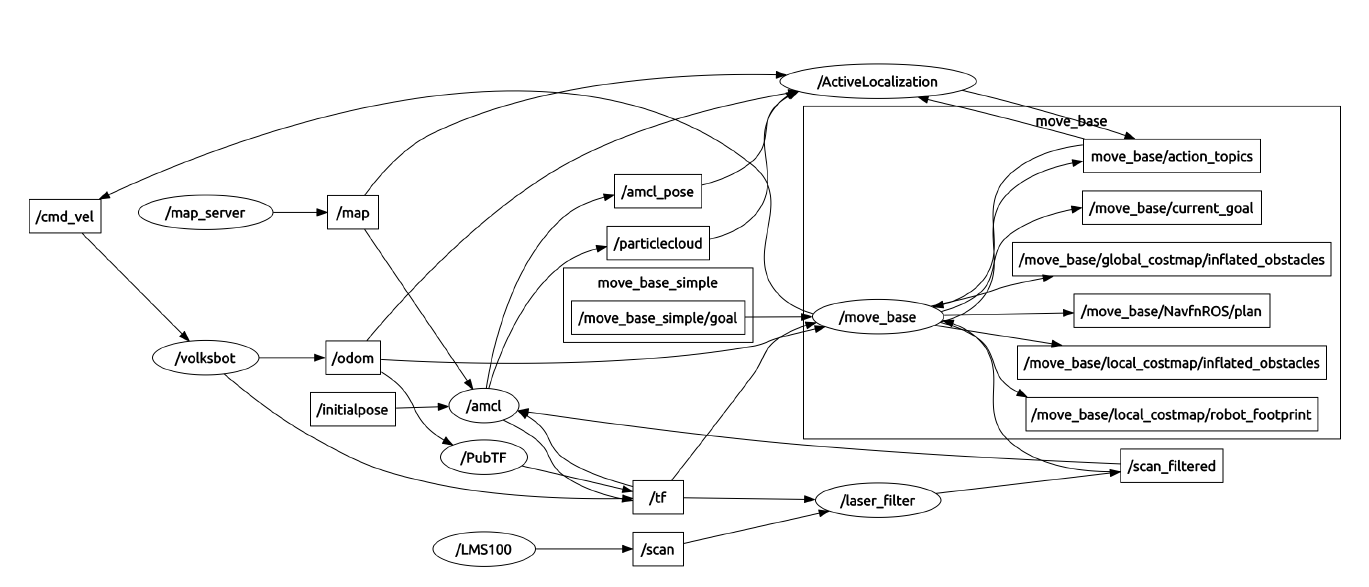
\includegraphics[width=1\textwidth]{figures/active_localization_node.png}
	\caption{An example of an active localization node}
	\label{fig:active_locnode}
\end{figure}


% underscore symbol {\_}


\fi